\label{sec:kszRecon}
The CMB temperature fluctuation caused by the kSZ effect is simply a line-of-sight integral of the free electron momentum field:
\begin{eqnarray}
\label{eq:ksz}
\Theta_\mr{kSZ}(\bm{n})\equiv\frac{\Delta T_\mr{kSZ}}{T_{\mr{CMB}}}
=-\frac{1}{c}\int d\eta  g(\eta)  p_\parallel(\eta,\bm{n})\ ,
\end{eqnarray}
where $\eta(z)$ is the comoving distance, $g(\eta)=e^{-\tau} d\tau/d\eta$ is the visibility function, $\tau$ is the optical depth to Thomson scattering, 
$p_\parallel=(1+\delta_e)v_\parallel$ is the momentum field parallel to the line of sight, and $\delta_e=(\rho-\bar{\rho})/\bar{\rho}$ is the free electron overdensity, with $\bar\rho$ denoting the average density. It is assumed that electron overdensity $\delta_e$ is closely related to baryon overdensity at $z<2$, therefore we simply use $\delta$ to denote both hereafter.

The direct correlation between kSZ and density fields vanishes due to the cancellation of positive and negative velocities. 
A holographic to avoid the cancellation is to reconstruct the peculiar velocity fields $v_z$ and convlove them with density fields at each redshift. 

From the linearized continuity equation:
\begin{eqnarray}
	\label{eq:v}
v_z(\bm{k})=i a H f\delta(\bm{k})\frac{k_z}{k^2}\,
\end{eqnarray}
where $a$ is the scale factor, $f=d\mathrm{ln}D/d\mathrm{ln}a$, $D(a)$ is the linear growth function, $H$ is the Hubble parameter, z is the direction 
parallel to the line of sight.

Now it is possible reconstruct the 2D kSZ field 
for a specific redshift bin 
with $v_z$ and $\delta$ following Eq (\ref{eq:ksz}). 
%In linear region, the continuity equation goes like:
%$\dot \delta+\nabla \cdot \bm{v}=0$, 
%where $\bm{v}$ is the peculiar velocity and $\delta$ is the matter overdensity. 
%Therefore, we obtain an estimator of velocity distribution from the density contract $\delta$:
%Therefore the real fields $v_z(\bm{x})$ contain mainly information of small k mode, large scale structure. 
%The linear theory works well in these scales.  
%(relative contributions of different scales in reverse Fourier transformation 
%indicated in Fig.\ref{fig:k3v}).
To quantify the tightness of correlation between reconstructed kSZ and real kSZ, 
we introduce a correlation coefficient $r$:
\begin{eqnarray}
\label{eq:r}
	r\equiv \frac{P_\mr{recon,real}}{\sqrt{P_\mr{recon}P_\mr{real}}}\,
\end{eqnarray}
where $P_\mr{recon,real}$ is the cross power spectrum.
%Where $\hat \Theta_\mr{kSZ}$ is reconstructed kSZ map, 
%and $\Theta_\mr{kSZ}$ is real kSZ map.

\begin{figure*}[btp]
\captionsetup{width=0.28\linewidth,justification=raggedright}
\begin{minipage}[t]{0.33\linewidth}
\begin{center}
\includegraphics[width=\textwidth,height=1.7\textwidth]{figure/k3pd_k3pv_z1_note.eps}
\end{center}
\vspace{-0.7cm}
\caption{
The variances $2\pi^2\Delta^2\equiv k^3P$ indicate how Fourier modes of different scales contribute to real space fields, i.e. $\delta(\bm{x})$ and $v_z(\bm{x})$. The modes essential for generating kSZ signals at $\ell\sim 500-3000$ are marked out as ``Golden modes''. 
}
\label{fig:k3v}
\end{minipage}
\begin{minipage}[t]{0.33\linewidth}
\begin{center}
\includegraphics[width=\textwidth,height=1.7\textwidth]{figure/powv2d_z1z2_r15r10.eps}
\end{center}
\vspace{-0.7cm}
\caption{The correlation coefficient between the reconstructed $v_z$  and actual $v_z$, assuming the longest baseline of 80 m with foregrounds seriously contaminate $k_z$ below $\sim0.08$ h/Mpc and $\sim0.12$ h/Mpc at $z=1~\&~2$, respectively}
\label{fig:v}
\end{minipage}
\begin{minipage}[t]{0.33\linewidth}
\begin{center}
\includegraphics[width=\textwidth,height=1.7\textwidth]{figure/powmomen_before_after_tide.eps}
\end{center}
\vspace{-0.7cm}
\label{fig:p}
\caption{The correlation coefficient between actual momentum fields $p_\parallel=(1+\delta)v_z$ and momentum fields reconstructed from 
IM fields before and 
after tidal reconstruction. 
The kSZ signal is roughly $p_\parallel$ integrated over line of sight, 
corresponding to $k_z=0$ modes. \philnote{Titles should say correlation coefficient of \dots or have no title.}}
\end{minipage}
\end{figure*}
